\begin{center}
	\line(1,0){70}
\end{center}

\paragraph{Question 2.1} Prove that allowing the certificate to be of size at \textit{most} $p(|x|)$ (rather than equal to $p(|x|)$) in Definition 2.1 makes no difference. That is, show that for every polynomial-time Turing machine $M$ and polynomial $p:\mathbb{N}\rightarrow\mathbb{N}$, the language
\begin{equation*}
	\{x:\exists |u| \text{ s.t. } u\leq p(|x|)\text{ and } M(x,u)=1\}
\end{equation*}
is in $\np$.

\paragraph{Answer.} We recall that a language $L\in\np$ iff there exists a polynomial $p$ and a polynomial-time TM $M$ such that for each $x\in\{0,1\}^{*}$,
\begin{equation*}
	x\in L\Leftrightarrow \exists u\in\{0,1\}^{p(|x|)}\text{ s.t. } M(x, u)=1.
\end{equation*}
We now need to show that the language given in the question (we can call it $L^{\leq}$) is in $\np$. To do this, we exhibit a polynomial $p^{\leq}$ and machine $M^{\leq}$ which satisfies the conditions outlined in the definition of $\np$. Set $p^{\leq}=p$ and let $M^{\leq}$ be the TM that on input $(x, u)$ where $u\in\{0,1\}^{p(|x|)}$ runs the machine $M$ on the first $i$ digits of $u$ for each $i\leq p(|x|)$ and accepts if $M$ accepts on any one of those inputs (otherwise it rejects). $M^{\leq}$ is a polynomial-time TM since $M$ is polynomial-time and it is run at most $p(|x|)$ times, where $p$ is polynomial. Now suppose $x\in L^{\leq}$. Then $\exists u$ which will be accepted by $M$, and it follows that $M^{\leq}$ accepts the string $u'$ which is $u$ padded until it is of length $p(|x|)$. Thus, $x\in L^{\leq}$ implies that $M^{\leq}$ accepts $(x,u)$ where $u$ is of length $p(|x|)$. Conversely, suppose that $M^{\leq}$ accepts some $(x, u)$ given as input. Then clearly $M$ accepts some $u'$ which consists of the first few digits of $u$. By definition, it follows that $x\in L$. We have shown both sides of the relation, and we are done.

\begin{center}
	\line(1,0){70}
\end{center}

\paragraph{Question 2.2} Prove that the following languages are in $\np$:
\begin{enumerate}
	\item \textit{Two Coloring:} $\mathsf{2COL}=\{G:\text{graph $G$ has a coloring with two colors}\}.$
	\item \textit{Three Coloring:} $\mathsf{3COL}=\{G:\text{graph $G$ has a coloring with three colors}\}.$
	\item \textit{Connectivity:} $\mathsf{CONNECTED}=\{G:\text{$G$ is a connected graph}\}.$
\end{enumerate}
Which ones of them are in $\p$?

\paragraph{Answer.} For simplicity purposes, we avoid dealing with turing machines.

\begin{enumerate}
	\item Two coloring is in $\np$. The witness for any graph is simply the labels of vertices colored blue. It can be checked whether each vertex has a blue label in polynomial time. A two-colorable graph is simply a bipartite graph, which is characterized by containing no cycles of odd length. We can detect odd cycles in a graph by traversing the graph using BFS and coloring each alternate layer with a different color. If during the procedure there is any vertex with a back-edge to the same color, the graph contains an odd cycle and is thus not in $\mathsf{2COL}$.
	\item Three coloring is again in $\np$ as the coloring serves as a witness. In fact, it is $\np$-complete. We will prove this in a later exercise.
	\item $\mathsf{CONNECTED}\in\np$ follows from $\mathsf{CONNECTED}\in\p$. The algorithm for checking connectivity is very simple: pick any vertex and traverse the graph. If the graph is disconnected, the traversal will terminate without touching all vertices.
\end{enumerate}

\begin{center}
	\line(1,0){70}
\end{center}

\paragraph{Question 2.3} Let $\mathsf{LINEQ}$ denote the set of satisfiable rational linear equations. That is, $\mathsf{LINEQ}$ consists of the set of all pairs $\langle A,b\rangle$ where $A$ is an $m\times n$ rational matrix and $b$ is an $m$-dimensional rational vector, such that $Ax=b$ for some $n$-dimensional vector $x$. Prove that $\mathsf{LINEQ}$ is in $\np$ (the key is to prove that if there exists such a vector $x$, then there exists an $x$ whose coefficients can be represented using a number of bits that is polynomial in the representation of $A, b$). (Note that $\mathsf{LINEQ}$ is actually in $\p$: Can you show this?)

\paragraph{Answer.} As the hint suggests, we have to show that there exists a witness $x$ for $\langle A, b\rangle$ which is of size polynomial in $|\langle A, b\rangle|$. 

The naive solution is that $\mathsf{LINEQ}$ is in $\np$ because it is in $\p$: in particular, the method of Gaussian Elimination converts $A$ into row-echelon form in polynomial time. After this, inspection can reveal the solution. This suffices to show that $\mathsf{LINEQ}\in\p\subseteq\np$.

The technique outlined in the hint only works for square matrices, and it proceeds as follows. We note that the determinant of $A$ is bounded by $n^2\left(\prod_{i,j=1}^{n}a_{ij}\right)$, the size of which is again polynomial in the representation of $\langle A, b\rangle$. It follows from Cramer's rule that the value of the $i^{\text{th}}$ variable is
\begin{equation*}
	x_i=\frac{\det(A_i)}{\det(A)}
\end{equation*}
where $A_i$ is $A$ except the $i^{\text{th}}$ column has been replaced by $b$; the determinant of this is again size-bounded polynomially due to similar considerations. It follows that a witness of polynomial size hence exists.

\begin{center}
	\line(1,0){70}
\end{center}

\paragraph{Question 2.4} Show that the $\mathsf{Linear}$ $\mathsf{Programming}$ ($\mathsf{LP}$) problem from Example 2.3 is in $\np$. (Again, this problem is actually in $\p$, though by a highly nontrivial algorithm.)

\paragraph{Answer.} Suppose that an instance $(A,b)$ of $\mathsf{LP}$ has a solution. We claim that the assignment of $x$ such that $Ax\leq b$ serves as a witness. As in 2.3, the only thing we have to do is show that $|x|$ is polynomially bounded in $|\langle A, b\rangle|$. Since $Ax\leq b$, $Ax=b'$ for some $b'\leq b$ (here $\leq$ is used to indicate that each $b_i'\leq b_i$). Then $x$ is also an assignment that satisifes the $\mathsf{LINEQ}$ instance $Ax=b'$, and is therefore bounded polynomially in $|\langle A,b'\rangle|$. Since $b'\leq b$, $|\langle A,b'\rangle|\leq|\langle A,b\rangle|$. Hence $|x|$ is also polynomially bounded in $|\langle A,b\rangle|$.

\begin{center}
	\line(1,0){70}
\end{center}

\paragraph{Question 2.5} Let $\mathsf{PRIMES}=\left\{n:n\text{ is prime}\right\}$. Show that $\mathsf{PRIMES}\in\np$. You can use the following fact: A number $n$ is prime iff for every prime factor $q$ of $n-1$, there exists a number $a\in\{2,\dots,n-1\}$ satisfying $a^{n-1}=1\pmod{n}$ but $a^{(n-1)/q}\neq 1\pmod n$.

\paragraph{Answer.} We note that the number of prime factors of $n$ is at most $\log n$. 

Assuming that we were provided a verified prime factorization $\mathcal{Q}$ of $n-1$, the set of numbers $\{a_q\}_{q\in\mathcal{Q}}$ corresponding to each prime that satisfies the property outlined in the question serves as a witness since we can easily perform modular exponentiation in polynomial time via repeated squaring. We cannot be certain, however, that any given prime factorization of $n-1$ is correct: we also have to show that each $q\in\mathcal{Q}$ is prime. First we note that $n-1$ must have $2$ as a prime factor. This is guaranteed since $n$ is odd (if $n=2$ we can just preprogram our algorithm to accept). It follows that any claimed prime factor $q$ is of size at most $(n-1)/2$, and the number of such prime factors is at most $\log n$; the size of the certificate is then polynomial in $n$.

To show that $q$ is prime, we can recursively give the same witness for $q$ that we gave for $n$; namely, a set of primes which multiply to $q-1$ and their corresponding `special' numbers, and then continue this process indefinitely. The various certificates compiled together form a witness if the number of tuples of the form $(q, a_q)$ is $O(\log n)$. We can show this is the case by induction: begin with $2$ and $3$, which is trivial, and then assume that for all primes up to some $k$ there is a witness of size $O(\log k)$. Then take the next prime $k'$ after $k$. Suppose $k'-1=p_1\dots p_m$. Then the size of the witness will be $1+m+\sum O(\log(p_i))=1+m+O(\log k')=O(\log k')$ since $m$ is at most $\log k'$, where we use the induction hypothesis in stating that each $p_i$ has a certificate of size $O(\log p_i)$ (by definition $p_i\leq k$). We thus conclude that for any prime $n$, a certificate of size $O(\log n)$ exists. We are done.

\begin{center}
	\line(1,0){70}
\end{center}

\paragraph{Question 2.7} Prove parts $2$ and $3$ of Theorem $2.8$.
\begin{enumerate}
	\item If language $L$ is $\np$-hard and $L\in\p$, then $p=\np$.
	\item If language $L$ is $\np$-complete, then $L\in\p$ iff $\p=\np$.
\end{enumerate}

\paragraph{Answer.} Our proofs proceed as follows.

\begin{enumerate}
	\item Let $L'$ be any arbitrary language in $\np$. We will show that $L'\in\p\implies\np\subseteq\p$. Combined with the fact that $\p\subseteq\np$, this is enough. Since $L$ is $\np$-hard, it follows that there exists a polyonmial-time computable function $f$ such that $x\in L\iff f(x)\in L'$. Then the following polytime algorithm for determining $x\in L'$ works: first, compute $f(x)$, and then run the algorithm for finding if $f(x)\in L'$. This is a polynomial time algorithm for the decision problem $x\in L'$, and it follows $L'\in\p$.
	\item Since $L$ is $\np$-hard, one side of the assertion follows from the previous part. The other side follows simply from the observation that if $\p=\np$ then $L\in\np\implies L\in\p$.
\end{enumerate}

\begin{center}
	\line(1,0){70}
\end{center}

\paragraph{Question 2.8} Let $\mathsf{HALT}$ be the Halting language defined in Theorem $1.11$. Show that $\mathsf{HALT}$ is $\np$-hard. Is it $\np$-complete?

\paragraph{Answer.} For $\mathsf{HALT}$ to be $\np$-complete, it would need to be in $\np$. However, this is clearly not true since $\mathsf{HALT}\notin\mathbf{EXP}$, as it cannot be determined by \textit{any} deterministic turing machine, and since $\np\subseteq\mathbf{EXP}$.

We will now show that $\mathsf{HALT}$ is $\np$-hard. Recall that $\mathsf{HALT}$ is the language consisting of the strings $\langle\alpha,x\rangle$ such that the TM $M_\alpha$ halts on $x$ within a finite number of steps. Let $L$ be any language in $\np$; by definition, there exists an $M$ such that $x\in L\iff M(x,u)=1$ for some $u\in \{0,1\}^{p(|x|)}$ where $p$ is a polynomial. We need to show that there is a polynomial-time computable function $f$ such that $x\in L\iff f(x)\in\mathsf{HALT}$. Let $M'$ be the machine that on input $x$ first calculates $p(|x|)$ and then runs $M(x,u)$ for increasing $u\in \{0,1\}^{p(|x|)}$, accepting if $M$ accepts and continuing to loop otherwise (it starts at $0^{p(|x|)}$ again if if it reaches $1^{p(|x|)}$). If $M'=M_\alpha$ for some $\alpha$, then $x\in L\iff \langle\alpha,x\rangle\in\mathsf{HALT}$. 

We can define the function $f$ which maps $x\mapsto\langle\alpha,x\rangle$. Constructing $\alpha$ is polynomial in $|x|$ since the description of $M$ is an independent constant, because $M=M_\beta$ for some $\beta$ which is invariant. We are done.

\begin{center}
	\line(1,0){70}
\end{center}

\paragraph{Question 2.9} We have defined a relation $\leq_p$ among languages. We noted that it is reflexive (i.e., $L \leq_p L$ for all languages $L$) and transitive (i.e., if $L\leq_p L'$ and $L'\leq_p L''$ then $L\leq_p L''$). Show that it is not symmetric, namely, $L\leq_p L'$ need not imply $L'\leq_p L$.

\paragraph{Answer.} The previous question provides an answer: every language $L\in\p$ is reducible to $\mathsf{HALT}$, but $\mathsf{HALT}$ is not reducible to any $\p$ problem since otherwise $\mathsf{HALT}$ would be polynomial-time solvable, which is false.

\begin{center}
	\line(1,0){70}
\end{center}

\paragraph{Question 2.10} Suppose $L_1, L_2\in\np$. Then is $L_1\cup L_2\in\np$? What about $\L_1\cap L_2$?

\paragraph{Answer.} Yes $L_1\cup L_2\in\np$. Consider the machine $M$, which takes an input $(x,u)$ and runs $M_1(x,u)$ and $M_2(x,u)$ and accepts iff at least one of $M_1$ or $M_2$ accept on the input, where $M_1$ and $M_2$ are the turing machines associated with $L_1$ and $L_2$ respectively. It follows that $x\in L_1\cup L_2\iff$ $\exists u\in\{0,1\}^{\leq p(|x|)}$ such that either $M_1(x,u)=1$ or $M_2(x,u)=1\iff$ $\exists u\in\{0,1\}^{\leq p(|x|)}$ such that $M(x,u)=1$.

$L_1\cap L_2\in\np$ follows from similar considerations, except $M$ now accepts iff both $M_1$ and $M_2$ accept. However, the two witnesses can be different, so we modify $M$ to run on a string $u\in\{0,1\}^{p(|x|)+q(|x|)}$ instead, where $p$ and $q$ are the polynomials corresponding to $L_1$ and $L_2$. Then if $\exists u_1, u_2$ which are accepted by $M_1$ and $M_2$ respectively, $M$ accepts $u_1||u_2$.

\begin{center}
	\line(1,0){70}
\end{center}

\paragraph{Question 2.11} Mathematics can be axiomatized using for example the Zermelo-Frankel system, which has a finite description. Argue at a high level that the following language is $\np$-complete. (You don't need to know anything about ZF.)
\begin{equation*}
	\mathsf{ZF}=\{\langle\varphi, 1^n\rangle:\text{math statement $\varphi$ has a proof of size at most $n$ in the ZF system}\}
\end{equation*}
The question of whether this language is in $\p$ is essentially the question asked by
Gödel in the chapter’s initial quote.

\paragraph{Answer.} A simple solution is to take a $\mathsf{SAT}$ instance $\phi$ and convert it in polynomial time to the statement $\varphi=$ ``there is a boolean assignment which satisfies $\phi$". Assuming that $\phi$ has $n$ variables, $\phi\in\mathsf{SAT}\iff\langle\varphi, 1^n\rangle\in \mathsf{ZF}$ since simply the assignment of bits in $\{0,1\}^n$ serves as a proof for $\varphi$. Since the function $f:\phi\mapsto\langle\varphi, 1^n\rangle$ is polytime computable, $\mathsf{SAT}\leq_p\mathsf{ZF}$, and we are done.

\begin{center}
	\line(1,0){70}
\end{center}

\paragraph{Question 2.12} Show that for every time constructible $T:\mathbb{N}\rightarrow\mathbb{N}$, if $L\in\mathbf{NTIME}(T(n))$, we can give a polynomial-time Karp reduction from $L$ to $\mathsf{3SAT}$ that transforms instances of size $n$ into 3CNF formulae of size $O(T(n)\log T(n))$. Can you make this reduction also run in $O(T(n)\poly(\log T(n)))$?

\paragraph{Answer.} The technical details of this proof are complicated and require explicit descriptions of Turing Machines, but since in this set of notes we avoid directly dealing with TM to the highest degree possible we skip this part which consists of checking that the `canonical' Cook-Levin reduction actually reduces $L$ to a CNF formula of size $O(T(n))$. To show that a 3CNF formula exists, we recall the CNF $\mapsto$ 3CNF transformation procedure: for each CNF unit of size $k$, split it into two parts and introduce the variable $z$ such that one side becomes $\vee z$ and the other becomes $\vee \bar{z}$. Keep doing this until you get units of size $3$; this transformation repeats $\log(T(n))$ times, and so the total length will be at most $O(T(n)\log(T(n)))$.

\begin{center}
	\line(1,0){70}
\end{center}

\paragraph{Question 2.13} Recall that a reduction $f$ from an $\np$-language $L$ to an $\np$-language $L'$ is \textit{parsimonious} if the number of certificates of $x$ is equal to the number of certificates of $f(x)$.
\begin{enumerate}
	\item[(a)] Prove that the reduction from every $\np$-complete language $L$ to $\mathsf{SAT}$ presented in the proof of Lemma 2.11 can be made parsimonious.
	\item[(b)] Show a parsimonious reduction from $\mathsf{SAT}$ to $\mathsf{3SAT}$.
\end{enumerate}

\paragraph{Answer.} Our proofs are as follows.

\begin{enumerate}
	\item[(a)] The reduction as given is already parsimonious \textbf{--} each `correct' string $(x,u)$ does get mapped to a correct execution of $M$ on it. Since the machine is deterministic, the final snapshot will be exactly the same because it has to be a function of the previous snapshots. In particular, there is only one correct execution of $M$ on $(x,u)$ which follows because there is actually only one execution of it. In this execution $z_{T(n)}$ will be the same every time, and it will be an accept state. The modification as given in the hint is not really required. The number of satisfying assignments of the CNF will be exactly equal to the number of witnesses.
	\item[(b)] The reduction works as follows. Take a CNF formula $C_1\wedge \dots\wedge C_n$ and suppose that any $C_i$ has more than three literals. Then replace $C_i=x_1\vee\dots\vee x_k$ with
	$$(x_1\vee x_2\vee z)\wedge(\bar{x_1}\vee\bar{z})\wedge(\bar{x_2}\vee\bar{z})\wedge(\bar{z}\vee\dots\vee x_k)$$
	Here we do the same thing as the reduction from $\mathsf{SAT}$ to $\mathsf{3SAT}$, except we force that $z=0$ if either $x_1$ or $x_2$ is nonzero.
\end{enumerate}

\begin{center}
\line(1,0){70}
\end{center}

\paragraph{Question 2.14} Cook used a somewhat different notion of reduction: A language $L$ is \textit{polynomial-time Cook reducible} to a language $L'$ if there is a polynomial time TM $M$ that, given an oracle for deciding $L'$, can decide $L$. An oracle for $L'$ is a magical extra tape given to $M$, such that whenever $M$ writes a single string on this tape and goes into a special ``invocation" state, then the string\textbf{--}in a single step!\textbf{--}gets overwritten by $1$ or $0$ depending on whether the string is or is not in $L'$; see section 3.4 for a more precise definition.

Show that the notion of cook reducibility is transitive and that $\mathsf{3SAT}$ is Cook-reducible to $\mathsf{TAUTOLOGY}$.

\paragraph{Answer.} We first show that Cook reducibility is transitive. Let $L\leq_C L'$ and let $L'\leq_C L''$. This means that there exists some $M$ which, given an oracle for $L'$, can solve $L$, and another $M'$ which, given an oracle for $L''$, can solve $L$. Then define the machine $M''$ as follows: on an input $x$, $M''$ simulates the action of $M$ until it needs to query an $L'$ instance. Instead of doing this, it writes down the instance on its work tape and simulates the action of $M'$ until it needs to query an $L''$ instance, which it does (when given an $L''$ oracle). Then it solves the $L'$ instance in polynomial time and returns to the original working on $x$. This machine is obviously polynomial time since $M$ and $M'$ are polynomial-time and can only query polynomially many oracles, and so $M''$ is a machine that shows that $L\leq_C L''$.

To show that $\mathsf{3SAT}$ is Cook-reducible to $\mathsf{TAUTOLOGY}$, it is enough to see that given $\varphi$, a machine $M$ can calculate $\bar{\varphi}$ and then query its $\mathsf{TAUTOLOGY}$ oracle on it. If $\varphi\in\mathsf{3SAT}\subseteq\mathsf{SAT}$, then by definition $\bar{\varphi}\in\overline{\sat}=\mathsf{TAUTOLOGY}$. If the oracle outputs $b$, then the machine can output $\bar{b}$, which is the solution to the $\mathsf{3SAT}$ instance.

\begin{center}
	\line(1,0){70}
\end{center}

\paragraph{Question 2.15} In the $\mathsf{CLIQUE}$ problem, we are given an undirected graph $G$ and an integer $K$ and have to decide whether there is a subset $S$ of at least $K$ vertices such that every two distinct vertices $u,v\in S$ have an edge between them (such a subset is called a \textit{clique} of $G$). In the $\mathsf{VERTEX COVER}$ problem, we are given an undirected graph $G$ and an integer $K$ and have to decide whether there is a subset $S$ of at most $K$ vertices such that for every edge $\overline{ij}$ of $G$, at least one of $i$ or $j$ is in $S$ (such a subset is called a \textit{vertex cover} of $G$). Prove that both of these problems are $\np$-complete.

\paragraph{Answer.} For $\mathsf{CLIQUE}$, it is enough to notice that if a graph $G$ has a clique of size $k$, then the complement graph $\bar{G}$ has an independent set of size $k$ (since all the members of the clique have edges to each other, in $\bar{G}$ none of them will have edges to each other). Thus given an $\mathsf{INDSET}$ instance, the machine can simply construct the complement graph in time $\binom{n}{2}$ which is a $\mathsf{CLIQUE}$ instance, and the function $f:G\mapsto\bar{G}$ forms a reduction to $\mathsf{INDSET}$ which is $\np$-complete.

For $\mathsf{VERTEXCOVER}$, begin with an $\mathsf{INDSET}$ instance $(G,k)$ and note that if there is an independent set $S$ of size $k$ then the set $V_G\setminus S$ of size $|V_{G}|-k$ forms a vertex cover \textbf{--} this immediately follows from the fact that since there are no edges between any elements of $S$, all the edges in the graph must be adjacent to some element of $V_G\setminus S$. Thus, the function $f:(G,k)\mapsto(G,n-k)$ forms a reduction from $\mathsf{VERTEXCOVER}$ to $\mathsf{INDSET}$.

\begin{center}
	\line(1,0){70}
\end{center}

\paragraph{Question 2.16} In the $\mathsf{MAXCUT}$ problem, we are given an undirected graph $G$ and an integer $K$ and have to decide whether there is a subset of vertices $S$ such that there are at least $K$ edges that have one endpoint in $S$ and one in $\bar{S}$. Prove this problem is $\np$-complete.

\paragraph{Answer.} We will show a reduction to $\mathsf{INDSET}$. Recall that this would involve converting an instance $x$ of $\mathsf{INDSET}$ to an instance $f(x)$ of $\mathsf{MAXCUT}$ such $x\in\mathsf{INDSET}\iff f(x)\in\mathsf{MAXCUT}$.

We begin with an instance $(G,k)$. Begin by adding an additional vertex $x$ to the graph, and connect $x$ to every vertex $v$. We will now replace each edge $(u,v)$ by a gadget $G_{(u,v)}$ which consists of:
\begin{enumerate}
	\item Four vertices, labelled $u,v, u'$ and $v'$.
	\item Edges $(x, u')$ and $(x,v')$.
	\item Edges $(u, u')$, $(v,v')$ and $(u',v')$.
\end{enumerate}
The final construction, $G'$, should look something like this. 

\begin{figure}[h]
	\centering
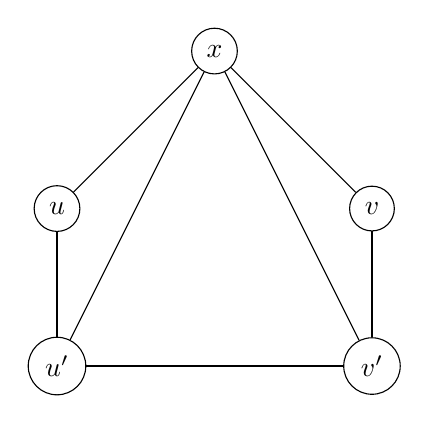
\begin{tikzpicture}
	\node[shape=circle,draw=black] (A) at (0,2) {$x$};
	\node[shape=circle,draw=black] (B) at (-2,0) {$u$};
	\node[shape=circle,draw=black] (C) at (2,0) {$v$};
	\node[shape=circle,draw=black] (D) at (-2,-2) {$u'$};
	\node[shape=circle,draw=black] (E) at (2,-2) {$v'$};
	
	\path (A) edge node[] {} (B);
	\path (A) edge node[] {} (C);
	\path (B) edge node[] {} (D);
	\path (C) edge node[] {} (E);
	\path (D) edge node[] {} (E);
	\path (A) edge node[] {} (D);
	\path (A) edge node[] {} (E);
\end{tikzpicture}
\end{figure}

We will now show that $G$ has an independent set of size at least $k$ iff $G'$ has a cut of size at least $4|E|+k$.

First, suppose $G$ has an independent set of size $k$; say it is $S$. Then we claim that the set $S'=S\cup\{v':u\in S,v\notin S\}\cup\{u',v':u,v\notin S\}$ is a cut of size at least $4|E|+k$. Begin by noting that for each gadget $G_{(u,v)}$ there are precisely $4$ edges which are in the cut regardless of whether $u$ or $v$ are in $S$. Thus there are at least $4|E|$ edges in the cut. Furthermore, $S$ is of size at least $k$, so there will be at least $k$ more edges in the cut of the form $(x,u)$. Hence there is a cut of at least $4|E|+k$ edges.

We will now show that if there is a cut in $G'$ of size at least $4|E|+k$, then there is an independent set of size at least $k$. Begin with the cut $S$, and assume that $x\notin S$ (if so, just consider $V\setminus S$). Let $I$ be the subset of $S$ which consists of vertices in $G$. We claim $I$ is the independent set we are looking for. Suppose to the contrary that $I$ is not independent; then there exist some $u,v\in I\subseteq S$ such that $(u,v)$ is an edge in $G$. Returning to $G'$, this means that since $u,v$ are both in $S$, at most $3$ edges of $G_{(u,v)}$ can be cut. Supposing that $m(I)$ is the number of edges in $I$, we can conclude that
$$|E(S)|\leq |I|+3m(I)+4(|E|-m(I))=|I|+|E|-m(I)$$
Since $|E(S)|\geq k+4|E|$, it implies that $|I|\geq k+m(I)$. The interpretation of this is that if each `extra' vertex is removed from the $m(I)$ edges in $I$, then the size will be at least $k$. But if it contains no edges, then $I$ is simply an independent set. We are done.

\begin{center}
	\line(1,0){70}
\end{center}

\paragraph{Question 2.17}

In the $\mathsf{EXACTLY}$ $\mathsf{ONE}$ $\mathsf{3SAT}$ (abbreviated $\mathsf{EO3SAT}$) we are given a 3CNF formula $\varphi$ and need to decide if there exists a satisfying assignment $u$ for $\varphi$ such that every clause of $\varphi$ has exactly one $\textsc{True}$ literal. In the $\mathsf{SUBSETSUM}$ problem, we are given a list of $n$ numbers $A_1,\dots,A_n$ and a number $T$ and need to decide whether there exists a subset $S\subseteq[n]$ such that $\sum_{i\in S} A_i=T$ (the problem size is the sum of all the bit representations of all numbers). Prove that both $\mathsf{EO3SAT}$ and $\mathsf{SUBSETSUM}$ are $\np$-complete.

\paragraph{Answer.} We will reduce $\mathsf{3SAT}$ to $\mathsf{EO3SAT}$. Start with a $\mathsf{3SAT}$ instance and consider any clause $C_i$, of the form $(x_{i,1}\vee x_{i,2}\vee x_{i,3})$. By introducing new variables $y_{i,j}$ and $z_{i,j}$, we can replace this clause by the following:
\begin{equation*}
	R=(z_{i,1}\vee z_{i,2}\vee z_{i,3})\wedge(x_{i,1}\vee y_{i,1}\vee z_{i,1})\wedge(x_{i,2}\vee y_{i,2}\vee z_{i,2})\wedge(x_{i,3}\vee y_{i,3}\vee z_{i,3})
\end{equation*}
Note that any solution to $(x_{i,1}\vee x_{i,2}\vee x_{i,3})$ admits an $\mathsf{EXACTLY}$ $\mathsf{ONE}$ solution to $R$ and any $\mathsf{EXACTLY}$ $\mathsf{ONE}$ solution to $R$ corresponds to a solution of $(x_{i,1}\vee x_{i,2}\vee x_{i,3})$. Since the transformation is polynomial in length, we have successfully reduced $\mathsf{3SAT}$ to $\mathsf{EO3SAT}$.

We will now reduce $\mathsf{SUBSETSUM}$ to $\mathsf{EO3SAT}$. Begin with an $\mathsf{EO3SAT}$ instance, and assign each literal the value $\sum_{x_i\in C_j}(2n)^j$, and set $T=\sum_{i=1}^{k}(2n)^i$ where the number of clauses is $k$. It is easy to see that this is a valid reduction.

\begin{center}
	\line(1,0){70}
\end{center}

\paragraph{Question 2.18} Prove that the language $\mathsf{HAMPATH}$ of undirected graphs with Hamiltonian paths is $\np$-complete. Prove that the language $\mathsf{TSP}$ described in Example 2.3 is $\np$-complete. Prove that the language $\mathsf{HAMCYCLE}$ of undirected graphs that contain Hamiltonian cycle (a simple cycle involving all the vertices) is $\np$-complete.

\paragraph{Answer.} We will reduce $\mathsf{HAMPATH}$ to $\mathsf{dHAMPATH}$. Consider any graph $G$ and create the new graph $G'$, which replaces each undirected edge $(u,v)$ with a pair of directed edges $\{(u,v),(v,u)\}$. It is easy to see that $G\in\mathsf{HAMPATH}\iff G'\in\mathsf{dHAMPATH}$.

For $\mathsf{TSP}$, it is easy to see that if we have a $\mathsf{HAMPATH}$ instance $G(V,E)$, then we can assign edge weights $w(e)=1$ if $e\in E$ and $w(e)=n+1$ otherwise. Then $G\in\mathsf{HAMPATH}\iff (G,n)\in\mathsf{TSP}$.

For $\mathsf{HAMCYCLE}$, we first show that $\mathsf{dHAMCYCLE}$ is $\np$-complete, which can be easily observed using the same reduction to $\sat$ with the exception that we connect the vertex $t$ and $s$ at the end, forming a complete cycle. Then $\mathsf{HAMCYCLE}$ reduces to $\mathsf{dHAMCYCLE}$ using the same technique as for $\mathsf{HAMPATH}$.
 
\begin{center}
	\line(1,0){70}
\end{center}

\paragraph{Question 2.19} Let $\mathsf{QUADEQ}$ be the langauge of all satisfiable sets of quadratic equations over 0/1 variables (a quadratic equation over $u_1,\dots u_n$ has the form $\sum_{i,j\in[n]}a_{i,j}u_iu_j=b)$ where addition is modulo 2. Show that $\mathsf{QUADEQ}$ is $\np$-complete.

\paragraph{Answer.} Consider any boolean formula in 3CNF form and let $C_i$ be some clause, say $(x\vee y\vee z)$. Then for each such clause, add the equations
\begin{align*}
	(1-x)(1-y)&=(1-w)\\
	(1-z)(1-w)&=0
\end{align*}
to the system. Each of these are of degree $2$, and the system has a solution in 0/1 iff the boolean formula has a solution. This is a reduction of $\mathsf{QUADEQ}$ to $\mathsf{SAT}$. Since the assignment is a witness for $\mathsf{QUADEQ}$, it is $\np$-complete.

\begin{center}
	\line(1,0){70}
\end{center}

\paragraph{Question 2.20} Let $\mathsf{REALQUADEQ}$ be the language of all satisfiable sets of quadratic equations over \textit{real} variables. Show that $\mathsf{REALQUADEQ}$ is $\np$-complete.

\paragraph{Answer.} Consider any system of equations which form a $\mathsf{QUADEQ}$ instance, and then simply add the constraint $x^2=x$ for each variable $x$. This is an instance of $\mathsf{REALQUADEQ}$ which has a solution iff each of the variables is 0/1 by the additional constraints. Then we have reduced $\mathsf{REALQUADEQ}$ to $\mathsf{QUADEQ}$.

\begin{center}
	\line(1,0){70}
\end{center}

\paragraph{Question 2.30} (Berman's Theorem 1978) A language is called \textit{unary} if every string in it is of the form $1^i$ (the string of $i$ ones) for some $i>0$. Show that if there exists an $\np$-complete unary language then $\p=\np$. (See Exercise 6.9 for a strengthening of this result.)

\paragraph{Answer.} Suppose there is some unary language $L$ that is $\np$-complete, and say that $\sat$ is reducible to it. We will show that using this fact we can solve $\sat$ in polynomial time, proving $\p=\np$.

Since we are dealing with polynomial-time reductions, we can assume that any $\sat$ instance $x$ can be reduced to an instance $f(x)$ of $L$ in time $p(|x|)$ for some polynomial $p$. Then it follows that $|f(x)|\leq p(|x|)$. Hence, $f(x)\in\{1^i:i\leq p(|x|)\}$. Recall that the number of $\sat$ instances of length $|x|$ is in fact $2^{|x|}$.

We now continue with a downward self-reducibility argument. Start with an instance $x$ and then substitute $x_1=0$ and $x_1=1$ respectively to get the formulas $\varphi_0$ and $\varphi_1$, and add the terms $(f(\varphi_i), \varphi_i)$ to a list. We then repeat the same procedure for $\varphi_i$ except that in case a term $(1^k, \varphi')$ appears more than once during the recursion we remove it. Keep repeating this in order of how the elements were added in the list. The list, on completion, will consist of a polynomial number of values, and will either contain $(f(\textsc{True}),\textsc{True})$ or not. If it does then $x\in\sat$, otherwise it isn't.

This is a polynomial-time algorithm for $\sat$, because the list we made is of polynomial size.

\begin{center}
	\line(1,0){70}
\end{center}

\paragraph{Question 2.31} Define the language $\mathsf{UNARYSUBSETSUM}$ to be the variant of the $\mathsf{SUBSETSUM}$ problem of Exercise 2.17 where all numbers are represented by the \textit{unary} representation (ie., the number $k$ is represented as $1^k$). Show that $\mathsf{UNARYSUBSETSUM}$ is in $\p$.

\paragraph{Answer.} The pseudopolynomial algorithm for $\mathsf{SUBSETSUM}$ works in time polynomial in the \textit{value} of the inputs. In unary, however, the value of each input is equal to the size. Thus the pseudopolynomial algorithm based on dynamic programming is polynomial in the size of the input, and so $\mathsf{UNARYSUBSETSUM}\in\p$.

\begin{center}
	\line(1,0){70}
\end{center}

\paragraph{Question 2.32} Prove that if every \textit{unary} $\np$-language is in $\p$ then $\mathbf{EXP}=\mathbf{NEXP}$. (A language $L$ is unary iff it is a subset of $\{1\}^{*}$, see Exercise 2.30.)

\paragraph{Answer.} Consider some $L\in\mathbf{NTIME}(2^{n^c})$. Then the language
$$\{\langle1^{|x|}, 1^{2^{|x|^c}}\rangle:x\in L\}$$
is in $\np$. Since it is in unary, by the assumption it is in $\p$ as well. However, there is a simple exponential-time algorithm which solves this: it simply lists down $\langle1^{|x|}, 1^{2^{|x|^c}}\rangle$ given an input $x$, then runs the polynomial time algorithm to determine whether it is in $L$. It follows that every language in $\mathbf{NEXP}$ is in $\mathbf{EXP}$, and we conclude that $\mathbf{NEXP}=\mathbf{EXP}$.

\begin{center}
	\line(1,0){70}
\end{center}

\paragraph{Question 2.33} Let $\Sigma_2\sat$ denote the following decision problem: Given a quantified formula $\psi$ of the form
\begin{equation*}
	\psi=\exists_{x\in\{0,1\}^n}\forall_{y\in\{0,1\}^m}\text{ s.t. }\varphi(x,y)=1
\end{equation*}
where $\varphi$ is a CNF formula, decide whether $\psi$ is true. That is, decide whether there exists an $x$ such that for every $y$, $\varphi(x, y)$ is true. Prove that if $\p=\np$, then $\Sigma_2\sat$ is in $\p$.

\paragraph{Answer.} Define the language $L(\varphi)$, where $x\in L(\varphi)$ iff $\forall_{y\in\{0,1\}^m}\varphi(x,y)=1$. Then by definition $L(\varphi)\in$ co$\np=\np=\p$. It follows that there exists a TM $M$ which takes in $(\psi, x)$ as an input and accepts depending on whether $x\in L(\varphi)$ which can be done in polynomial time. However, this is an $\np$-machine with $x$ as a witness to $\psi$, so $\Sigma_2\sat$ must be in $\np$. However since $\np=\p$, we can conclude that $\Sigma_2\sat\in\p$.

\begin{center}
	\line(1,0){70}
\end{center}

\paragraph{Question 2.34} Suppose that you are given a graph $G$ and a number $K$ and are told that either (i) the smallest vertex cover (see Exercise 2.15) of $G$ is of size at most $K$ or (ii) it is of size at least $3K$. Show a polynomial-time algorithm that can distinguish between these two cases. Can you do it with a smaller constant than $3$? Since $\mathsf{VERTEX COVER}$ is $\np$-hard, why does this algorithm not show that $\p=\np$?

\paragraph{Answer.} The greedy algorithm for vertex cover (that selects the highest-degree vertex and adds it to the cover) is a $2$-approximation, and so simply running the algorithm and checking whether the returned cover is of size $2K$ or less is enough. 

The smallest constant it can be done with is $2$, since the greedy algorithm is a $2$-approximation. It can potentially be done with an even smaller constant assuming that we have a better approximation.

The algorithm does not show $\p=\np$ because ultimately it does not solve vertex cover, it simply approximates it.
